\section{Iterated Integrals} \label{S:11.2.Iterated_Integrals}

\vspace*{-14 pt}
\framebox{\hspace*{3 pt}
\parbox{6.25 in}{\begin{goals}
\item How do we evaluate a double integral over a rectangle as an iterated integral, and why does this process work?
\end{goals}} \hspace*{3 pt}}



\subsection*{Introduction}

Recall that we defined the double integral of a continuous function $f = f(x,y)$ over a rectangle $R = [a,b] \times [c,d]$ as
\[\iint_R f(x,y) \, dA = \lim_{m,n \to \infty} \sum_{j=1}^n \sum_{i=1}^m f\left(x_{ij}^*, y_{ij}^*\right) \cdot \Delta A,\]
where the different variables and notation are as described in Section~\ref{S:11.1.Double_Integrals_Rectangles}.  Thus $\iint_R f(x,y) \, dA$ is a limit of double Riemann sums, but while this definition tells us exactly what a double integral is, it is not very helpful for determining the value of a double integral. Fortunately, there is a way to view a double integral as an \emph{iterated integral}\index{iterated integral!rectangular coordinates}, which will make computations feasible in many cases.

The viewpoint of an iterated integral is closely connected to an important idea from single-variable calculus.  When we studied solids of revolution, such as the one shown in Figure~\ref{F:6.2.Ex1}, we saw that in some circumstances we could slice the solid perpendicular to an axis and have each slice be approximately a circular disk.  From there, we were able to find the volume of each disk, and then use an integral to add the volumes of the slices.  In what follows, we are able to use single integrals to generalize this approach to handle even more general geometric shapes.

\begin{figure}[h]
\begin{center}
%\includegraphics{figures/6_2_Ex1.eps}
  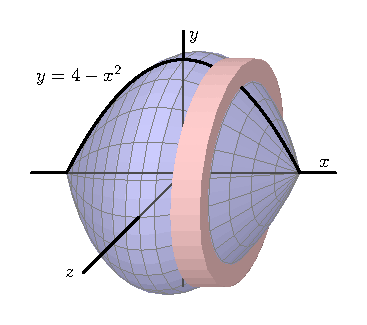
\includegraphics{figures/fig_11_2_volume_revolve.eps}
\caption{A solid of revolution.} \label{F:6.2.Ex1}
\end{center}
\end{figure}

%\begin{itemize}
%\item $x_0$, $x_1$, $\ldots$, $x_m$ are the endpoints of $m$ equal length subintervals of $[a,b]$ of length $\Delta x = \frac{b-a}{m}$ with $a = x_0<x_1<x_2 < \cdots < x_m = b$;
%\item $y_0$, $y_1$, $\ldots$, $y_n$ are the endpoints of $n$ equal length subintervals of $[c, d]$ of length $\Delta y = \frac{d-c}{n}$ with $c = y_0<y_1<y_2 < \cdots < y_n = d$;
%\item $R_{ij} = [x_{i-1},x_{i}] \times [y_{j-1}, y_j]$ is the subrectangle of $R$ with opposite vertices $(x_{i-1},y_{j-1})$ and $(x_i, y_j)$ for $i$ between $1$ and $m$ and $j$ between $1$ and $n$. The area of $R_{ij}$ is $\Delta A = \Delta x \cdot \Delta y$;
%\item $(x_{ij}^*, y_{ij}^*)$ is a point in rectangle $R_{ij}$.
%\end{itemize}



\begin{pa} \label{PA:11.2} Let $f(x,y) = 25-x^2-y^2$ on the rectangular domain $R = [-3,3] \times [-4,4]$.

As with partial derivatives, we may treat one of the variables in $f$ as constant and think of the resulting function as a function of a single variable. Now we investigate what happens if we integrate instead of differentiate.

	\ba
	\item  Choose a fixed value of $x$ in the interior of $[-3,3]$. Let
\[A(x) = \int_{-4}^4 f(x,y) \, dy.\]
What is the geometric meaning of the value of $A(x)$ relative to the surface defined by $f$. (Hint: Think about the trace determined by the fixed value of $x$, and consider how $A(x)$ is related to Figure \ref{F:11.2.Cross_section_PA_y}.)
\begin{figure}[ht]
\begin{center}
\begin{minipage}{2.5in}
\begin{center}
%\resizebox{!}{2.4in}{\includegraphics[trim=0cm 0cm 0.25cm 0.5cm,clip]{11_2_Cross_section_PA_y}}
  \includegraphics{figures/fig_11_2_preview_slice.eps}
\end{center}
\caption{A cross section with fixed $x$.}
\label{F:11.2.Cross_section_PA_y}
\end{minipage} \hspace{0.2in}
\begin{minipage}{2.5in}
\begin{center}
%\resizebox{!}{2.4in}{\includegraphics[trim=0cm 0cm 0.25cm 0.5cm,clip]{11_2_Cross_section_PA_y_slab}}
  \includegraphics{figures/fig_11_2_preview_thick.eps}
\end{center}
\caption{A cross section with fixed $x$ and $\Delta x$.}
\label{F:11.2.Cross_section_PA_y_slab}
\end{minipage}
\end{center}
\end{figure}
%crop graphics in animate trim=<left> <bottom> <right> <top>, add, clip with \includegraphics



  	\item For a fixed value of $x$, say $x_i^*$, what is the geometric meaning of $A(x_i^*) \ \Delta x$?  (Hint: Consider how $A(x_i^*) \Delta x$ is related to Figure \ref{F:11.2.Cross_section_PA_y_slab}.)


	\item Since $f$ is continuous on $R$, we can define the function $A = A(x)$ at every value of $x$ in $[-3,3]$. Now think about subdividing the $x$-interval $[-3,3]$ into $m$ subintervals, and choosing a value $x_i^*$ in each of those subintervals.  What will be the meaning of the sum $\ds \sum_{i=1}^m A(x_i^*) \ \Delta x$? 


	\item Explain why $\int_{-3}^3 A(x) \, dx$ will determine the exact value of the volume under the surface $z = f(x,y)$ over the rectangle $R$.
%\int_{-3}^3 \left( \int_{-4}^4 f(x,y) \, dy \right) \, dx\]
%The latter integral is an \emph{iterated integral}.


	\ea
\end{pa} 

\begin{activitySolution}
	\ba
	\item  Since $f(x,y) \geq 0$ on the given domain, the value of $A(x)$ tells us the area under the $y$-trace curve for that fixed value of $x$.

  	\item Since $A(x_i^*)$ is an area under the $y$-trace for the value $x = x_i^*$, when we multiply that area by a constant width $\Delta x$, we obtain the volume of a slab obtained by thickening the region under the $x=x_i^*$ trace by a uniform thickness $\Delta x$.


	\item This sum will give us the sum of volumes of slabs with constant cross sections parallel to the $yz$-plane, where the cross sections look like the areas under the graphs of the $x_i^*$ traces. 


	\item As we let $m$ go to infinity, the thickness of the slabs goes to 0 and we are just adding up all of the cross sectional areas of the surface parallel to the $yz$-plane, and so 
\[\int_{-3}^3 A(x) \, dx = \lim_{m \to \infty} \sum_{i=1}^m A(x_i^*) \ \Delta x\]
gives us the volume of the solid under the surface $z = f(x,y)$ over the rectangle $R$.

	\ea

\end{activitySolution}

\afterpa 

\subsection*{Iterated Integrals}

The ideas that we explored in Preview Activity \ref{PA:11.2} work more generally and lead to the idea of an iterated integral. Let $f$ be a continuous function on a rectangular domain $R = [a,b] \times [c,d]$, and let
\[A(x) = \int_c^d f(x,y) \, dy.\]
The function $A = A(x)$ determines the value of the cross sectional area\footnote{By area we mean ``signed" area.} in the $y$ direction for the fixed value of $x$ of the solid bounded between the surface defined by $f$ and the $xy$-plane.

\begin{figure}[ht]
\begin{center}
%\resizebox{!}{3.0in}{\animategraphics[controls,trim=0cm 0.25cm 0.1cm 1.0cm]{4}{11_2_II_}{01}{05}}
%\animategraphics[controls]{6}{figures/fig_11_2_preview_animate_}{0}{5}
\resizebox{!}{1.5in}{\includegraphics{figures/fig_11_2_preview_animate_0.pdf}} \hspace{0.25in} \resizebox{!}{1.5in}{\includegraphics{figures/fig_11_2_preview_animate_2.pdf}} \hspace{0.25in} \resizebox{!}{1.5in}{\includegraphics{figures/fig_11_2_preview_animate_5.pdf}}
\end{center}
\caption{Summing cross section slices.}
\label{F:11.2.Cross_section_y_slab_sum}
\end{figure}
%crop graphics in animate trim=<left> <bottom> <right> <top>, add, clip with \includegraphics

The value of this cross sectional area is determined by the input $x$ in $A$. Since $A$ is a function of $x$, it follows that  we can integrate $A$ with respect to $x$. In doing so, we use a partition of $[a, b]$ and make an approximation to the integral given by
\[\int_a^b A(x) \, dx  \approx \sum_{i=1}^m A(x_i^*) \Delta x,\]
where $x_i^*$ is any number in the subinterval $[x_{i-1},x_i]$. Each term $A(x_i^*) \Delta x$ in the sum represents an approximation of a fixed cross sectional slice of the surface in the $y$ direction with a fixed width of $\Delta x$ as illustrated in Figure \ref{F:11.2.Cross_section_PA_y_slab}. We add the signed volumes of these slices as shown in the frames in Figure \ref{F:11.2.Cross_section_y_slab_sum} to obtain an approximation of the total signed volume.

As we let the number of subintervals in the $x$ direction approach infinity, we can see that the Riemann sum $\ds \sum_{i=1}^m A(x_i^*) \Delta x$
approaches a limit and that limit is the sum of signed volumes bounded by the function $f$ on $R$. Therefore, since $A(x)$ is itself determined by an integral, we have
\[\iint_R f(x,y) \, dA = \lim_{m \to \infty} \sum_{i=1}^m A(x_i^*) \Delta x = \int_a^b A(x) \, dx = \int_a^b \left( \int_c^d f(x,y) \, dy \right) \, dx.\]

Hence, we can compute the double integral of $f$ over $R$ by first integrating $f$ with respect to $y$ on $[c, d]$, then integrating the resulting function of $x$ with respect to $x$ on $[a, b]$. The nested integral
\[\int_a^b \left( \int_c^d f(x,y) \, dy \right) \, dx = \int_a^b \int_c^d f(x,y) \, dy \, dx \]
is called an \emph{iterated integral}, and we see that each double integral may be represented by two single integrals.

We made a choice to integrate first with respect to $y$. The same argument shows that we can also find the double integral as an iterated integral integrating with respect to $x$ first, or
\[\iint_R f(x,y) \, dA = \int_c^d \left( \int_a^b f(x,y) \, dx \right) \, dy = \int_c^d  \int_a^b f(x,y) \, dx  \, dy.\]

The fact that integrating in either order results in the same value is known as Fubini's Theorem.

\vspace*{5pt}
\nin \framebox{\hspace*{3 pt}
\parbox{6.25 in}{\textbf{Fubini's Theorem.} If $f = f(x,y)$ is a continuous function on a rectangle $R = [a,b] \times [c,d]$, then
\[\iint_R f(x,y) \, dA = \int_c^d \int_a^b f(x,y) \, dx \, dy = \int_a^b \int_c^d f(x,y) \, dy \, dx.\]
} \hspace*{3 pt}}
\vspace*{5pt}

Fubini's theorem enables us to evaluate iterated integrals without resorting to the limit definition.  Instead, working with one integral at a time, we can use the Fundamental Theorem of Calculus from single-variable calculus to find the exact value of each integral, starting with the inner integral.

\begin{activity} \label{A:11.2.1} Let $f(x,y) = 25-x^2-y^2$ on the rectangular domain $R = [-3,3] \times [-4,4]$.
	\ba
	\item Viewing $x$ as a fixed constant, use the Fundamental Theorem of Calculus to evaluate the integral 
	\[A(x) = \int_{-4}^4 f(x,y) \, dy.\]
Note that you will be integrating with respect to $y$, and holding $x$ constant.  Your result should be a function of $x$ only.

	\item Next, use your result from (a) along with the Fundamental Theorem of Calculus to determine the value of $\ds \int_{-3}^3 A(x) \, dx$.
		
	\item What is the value of $\ds \iint_R f(x,y) \, dA$? What are two different ways we may interpret the meaning of this value?
	
	\ea

\end{activity}
\begin{smallhint}

\end{smallhint}
\begin{bighint}

\end{bighint}
\begin{activitySolution}
	\ba
	\item Treating $x$ as a constant we have 
\begin{align*}
A(x) &= \int_{-4}^4 f(x,y) \, dy \\
	&= \int_{-4}^4 25-x^2-y^2 \, dy \\
	&= \left. \left[ (25-x^2)y - \frac{y^3}{3} \right] \right|_{-4}^4 \\
	&= 8(25-x^2) - \frac{128}{3} \\
	&= \frac{472}{3} - 8x^2.
\end{align*}

	\item Then
\begin{align*}
\int_{-3}^3 A(x) \, dx &= \int_{-3}^3 \frac{472}{3} - 8x^2 \, dx \\
	&= \left. \left[ \frac{472}{3}x - \frac{8}{3}x^3 \right] \right|_{-3}^3 \\
	&= 944 - 144 \\
	&= 800.
\end{align*}
	
	\item Using the results of parts (a) and (b) we have 
\[\iint_R f(x,y) \, dA = \int_{-3}^3 \int_{-4}^4 f(x,y) \, dy \, dx = 800.\]
Since $f(x,y) \geq 0$ on $R$, this result tells us that the volume of the solid bounded above the graph of $f$ and below by the rectangle $R$ is 800. The area of $R$ is 48, so this result also tells us that the average value of $f$ on $R$ is $\frac{800}{48}$. 
	
	
	
	\ea
\end{activitySolution}
\aftera


\begin{activity} \label{A:11.2.2} Let $f(x,y) = x+y^2$ on the rectangle $R = [0,2] \times [0,3]$.
	\ba
	\item Evaluate $\ds \iint_R f(x,y) \, dA$ using an iterated integral.  Choose an order for integration by deciding whether you want to integrate first with respect to $x$ or $y$.  
	
	\item Evaluate $\ds \iint_R f(x,y) \, dA$ using the iterated integral whose order of integration is the opposite of the order you chose in (a).	
	
	\ea

\end{activity}
\begin{smallhint}

\end{smallhint}
\begin{bighint}

\end{bighint}
\begin{activitySolution}
	\ba
	\item We evaluate $\ds \iint_R f(x,y) \, dA$ as an iterated integral, integrating first with respect to $x$, then $y$:
	\begin{align*}
	 \iint_R f(x,y) \, dA &=  \int_{0}^{3} \int_{0}^{2} x+y^2 \, dx \, dy \\
		&= \int_{0}^{3} \left. \left[ \frac{x^2}{2} + xy^2 \right] \right|_{0}^{2}  \, dy \\
		&= \int_{0}^{3} \left[ 2 + 2y^2 \right]  \, dy \\
		&= \left. \left[ 2y + \frac{2}{3}y^3 \right] \right|_{0}^{3} \\
		&= 24.
	\end{align*}
	
	
	
	\item We evaluate $\ds \iint_R f(x,y) \, dA$ as an iterated integral, integrating first with respect to $y$, then $x$:
	\begin{align*}
	 \iint_R f(x,y) \, dA &=  \int_{0}^{2} \int_{0}^{3} x+y^2 \, dy \, dx \\
		&= \int_{0}^{2} \left. \left[ xy + \frac{y^3}{3} \right] \right|_{0}^{3}  \, dx \\
		&= \int_{0}^{2} \left[ 3x + 9 \right]  \, dx \\
		&= \left. \left[ \frac{3}{2}x^2 + 9x \right] \right|_{0}^{2} \\
		&= 24.
	\end{align*}
	\ea
\end{activitySolution}
\aftera


\begin{summary}	
\item We can evaluate the double integral $\ds \iint_R f(x,y) \, dA$ over a rectangle $R = [a,b] \times [c,d]$ as an iterated integral in one of two ways:
    \begin{itemize}
    \item[-] $\ds \int_a^b \left( \int_c^d f(x,y) \, dy \right) \, dx$, or
    \item[-] $\ds \int_c^d \left( \int_a^b f(x,y) \, dx \right) \, dy$.
    \end{itemize}
This process works because each inner integral represents a cross-sectional (signed) area and the outer integral then sums all of the cross-sectional (signed) areas.  Fubini's Theorem guarantees that the resulting value is the same, regardless of the order in which we integrate.
\end{summary}


\nin \hrulefill

\begin{exercises} 

\item Evaluate each of the following double or integrated integrals exactly.
\ba
	\item $\ds \int_1^3 \left( \int_2^5 xy \, dy \right) \, dx$
	\item $\ds \int_0^{\pi/4} \left( \int_0^{\pi/3} \sin(x) \cos(y) \, dx \right) \, dy$
	\item $\ds \int_0^1 \left( \int_0^1 e^{-2x - 3y} \, dy \right) \, dx$
	\item $\ds \iint_R \sqrt{2x + 5y} \, dA$, where $R = [0,2]\times[0,3]$.
\ea

\begin{exerciseSolution}
\ba
	\item We integrate first with respect to $y$, then with respect to $x$:
\begin{align*}
\int_1^3 \left( \int_2^5 xy \, dy \right) \, dx &= \int_1^3 \left( x\frac{y^2}{2}\right)\biggm|_{y=2}^{5} \, dx \\
	&= \int_1^3  \frac{21}{2}x \, dx  \\
	&= \frac{21}{4}x^2 \biggm|_{x=1}^3 \\
	&= \frac{21}{4}(8) \\
	&= 42.
\end{align*}

	\item We integrate first with respect to $x$, then with respect to $y$:
\begin{align*}
\int_0^{\pi/4} \left( \int_0^{\pi/3} \sin(x) \cos(y) \, dx \right) \, dy &= \int_0^{\pi/4} \left( -\cos(x) \cos(y) \biggm|_0^{x=\pi/3}  \right) \, dy  \\
	&= \int_0^{\pi/4} \left( -\frac{1}{2}-(-1)\right) \cos(y) \, dy  \\
	&= \frac{1}{2} \sin(y) \biggm|_{y=0}^{\pi/4} \\
	&= \frac{\sqrt{2}}{4}.
\end{align*}

	\item We integrate first with respect to $y$, then with respect to $x$:
\begin{align*}
\int_0^1 \left( \int_0^1 e^{-2x - 3y} \, dy \right) \, dx &= \int_0^1 \left( -\frac{1}{3}e^{-2x - 3y}\biggm|_{y=0}^1 \right) \, dx  \\
	&= -\frac{1}{3} \int_0^{1} \left( e^{-2x-3} - e^{-2x} \right) \, dy  \\
	&= \frac{1}{6} \left(e^{-2x-3} - e^{-2x}\right) \biggm|_{x=0}^{1} \\
	&= \frac{\sqrt{1}}{6} \left(e^{-5}-e^{-2} - e^{-3} + 1\right).
\end{align*}

	\item We integrate first with respect to $y$, then with respect to $x$:
\begin{align*}
\iint_R \sqrt{2x + 5y} \, dA &= \int_0^2 \left( \int_0^3 \sqrt{2x+5y} \, dy \right) \, dx \\
	&= \int_0^2 \left( \frac{2}{15}(2x+5y)^{3/2}\biggm|_{y=0}^3 \right) \, dx \\
	&= \frac{2}{15}\int_0^2 \left( (2x+15)^{3/2} - (2x)^{3/2} \right) \, dx \\
	&= \left(\frac{2}{15}\right)\left(\frac{1}{5}\right) \left( (2x+15)^{5/2} - (2x)^{5/2} \right)\biggm|_{x=0}^2  \\
	&= \frac{2}{75} \left(19^{5/2} - 4^{5/2} - 15^{5/2}\right).
\end{align*}
\ea
\end{exerciseSolution}

\item The temperature at any point on a metal plate in the $xy$ plane is given by $T(x,y) = 100-4x^2 - y^2$, where $x$ and $y$ are measured in inches and $T$ in degrees Celsius.  Consider the portion of the plate that lies on the rectangular region $R = [1,5] \times [3,6]$.

\ba
	\item Write an iterated integral whose value represents the volume under the surface $T$ over the rectangle $R$. 
	\item Evaluate the iterated integral you determined in (a).
	\item Find the area of the rectangle, $R$.
	\item Determine the exact average temperature, $T_{\mbox{\tiny{AVG}(R)}}$, over the region $R$.
\ea

\begin{exerciseSolution}
\ba
	\item An iterated integral whose value represents the volume under the surface $T$ over the rectangle $R$ is
\[\int_1^5 \left( \int_3^6 100 - 4x^2-y^2 \, dy \right) \, dx.\]

	\item Integrating with respect to $y$ then $x$ gives us
\begin{align*}
\int_1^5 \left( \int_3^6 100 - 4x^2-y^2 \, dy \right) \, dx &= \int_1^5 \left( (100-4x^2)y - \frac{y^3}{3} \right)\biggm|_3^6  \, dx \\
	&= \int_1^5 \left( 300-12x^2 - \frac{189}{3} \right) \, dx \\
	&= \left( 300x-4x^3 - \frac{189}{3}x \right)\biggm|_1^5  \\
	&= 1200 - 496 - \frac{756}{3} \\
	&= 452.
\end{align*}

	\item The area of the rectangle, $R$, is $(4)(3) = 12$. 
	
	\item The exact average temperature, $T_{\mbox{\tiny{AVG}(R)}}$, over the region $R$ is
\[T_{\mbox{\tiny{AVG}(R)}} = \frac{1}{\text{Area}(R)} \iint_R T(x,y) \, dA = \frac{452}{12} = \frac{113}{3}.\]

\ea
\end{exerciseSolution}

\item Consider the box with a sloped top that is given by the following description:  the base is the rectangle $R = [1,4] \times [2,5]$, while the top is given by the plane $z = p(x,y) = 30 - x - 2y$.

\ba
	\item Write an iterated integral whose value represents the volume under $p$ over the rectangle $R$. 
	\item Evaluate the iterated integral you determined in (a).
	\item What is the exact average value of $p$ over $R$?
	\item If you wanted to build a rectangular box (with an identical base) that has the same volume as the box with the sloped top described here, how tall would the rectangular box have to be?
\ea

\begin{exerciseSolution}
\ba
	\item An iterated integral whose value represents the volume under $p$ over the rectangle $R$ is
\[\int_1^4 \left( \int_2^5 30-x-2y \, dy \right) \, dx.\] 

	\item Integrating with respect to $y$ then $x$ gives us
\begin{align*}
\int_1^4 \left( \int_2^5 30-x-2y \, dy \right) \, dx &= \int_1^4 \left( (30-x)y - y^2 \right)\biggm|_2^5 \, dx \\
	&= \int_1^4 \left( 90-3x - 21 \right) \, dx \\
	&= \left( 69x-\frac{3}{2}x^2 \right)\biggm|_1^4  \\
	&= 207 - \frac{45}{2}  \\
	&= 184.5.
\end{align*}

	\item The exact average value of $p$ over $R$ is 
\[p_{\mbox{\tiny{AVG}(R)}} = \frac{1}{\text{Area}(R)} \iint_R p(x,y) \, dA = \frac{184.5}{(3)(3)} = 20.5.\]
	\item The average value of $p$ over $R$ tells us the height of a rectangular box (with an identical base) that has the same volume as the box with the sloped top described here, so we need a box of height $20.5$. 
\ea
\end{exerciseSolution}


\end{exercises} 

\afterexercises


\clearpage
